\documentclass[10pt]{beamer}

\usetheme[progressbar=frametitle]{metropolis}
\usepackage{appendixnumberbeamer}
\usepackage{booktabs}
\usepackage[scale=2]{ccicons}

\usepackage{pgfplots}
\usepgfplotslibrary{dateplot}

\usepackage{xspace}
\newcommand{\themename}{\textbf{\textsc{metropolis}}\xspace}
\newcommand{\setbra}[1]{\left\{#1\right\}}
\newcommand{\set}[1]{\setbra{#1}}
\newcommand{\bra}[1]{\left[#1\right]}
\newcommand{\pa}[1]{\left(#1\right)}
\newcommand{\abs}[1]{\left| #1\right|}
\newcommand{\norm}[1]{\left\| #1 \right\|}
\newcommand{\angs}[1]{\left\langle #1\right\rangle}
\newcommand{\midvert}{\middle|}

\newcommand{\E}{\mathbb{E}}

\title{Output Dynamics in Real-Business-Cycle Models}
\subtitle{Timothy Cogley and James M. Nason}
\date{\today}

\author{Zixuan, Huixin, Rémi}
\institute{M2 ETE Macroeconomics 2}

\begin{document}

\maketitle

\begin{frame}{Table of contents}
    \setbeamertemplate{section in toc}[sections numbered]
    \tableofcontents%[hideallsubsections]
\end{frame}

\section{Introduction}

\begin{frame}{Introduction}
    \textit{Are RBC models consistent with output dynamics stylized facts?}\\
    $\Rightarrow$ Compare \alert{output dynamics} in the theoretical RBC model literature and \alert{stylized facts} in the output dynamics analysis\\[1em]

    \begin{itemize}
        \item Stylized fact \#1: \alert{Autocorrelation} for output growth
              \begin{itemize}
                  \item Short horizons: \textbf{Positive and significant}
                  \item Long horizons: \textbf{Negative but insignificant}
              \end{itemize}
    \end{itemize}
    \begin{figure}
        \centering
        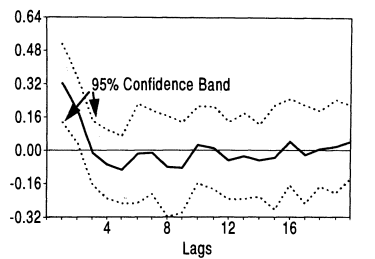
\includegraphics[width=5cm]{figures/sf1.png}
        \caption{Autocorrelation function for output growth}
    \end{figure}
\end{frame}

\begin{frame}{Introduction}
    \begin{itemize}
        \setlength\itemsep{1em}
        \item Stylized fact \#2: \alert{Impulse-response functions} of output
              \begin{itemize}
                  \item \textbf{Permanent shock} $\varepsilon_z$: Output $\uparrow$ then reaches a plateau
                  \item \textbf{Transitory shock} $\varepsilon_g$: Output $\uparrow$ then goes back to stochastic trend
                  \item Variation in GNP growth: mainly due to transitory fluctuation
                  \item[$\Rightarrow$] GNP: important \alert{trend-reverting component}
              \end{itemize}
    \end{itemize}
    \begin{figure}
        \centering
        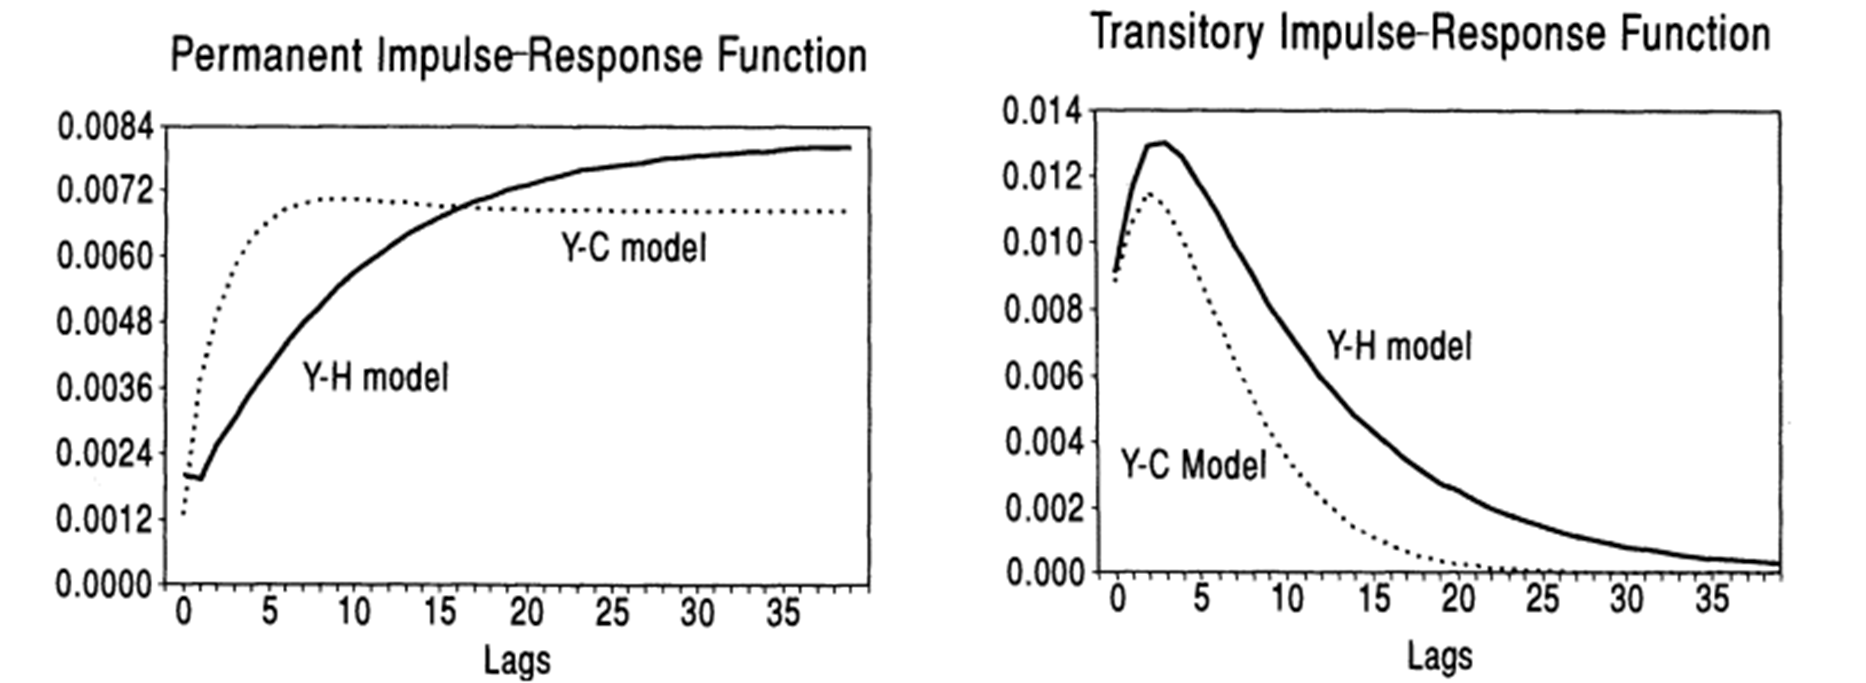
\includegraphics[width=10cm]{figures/sf2.png}
        \caption{Impulse-response functions for output growth}
    \end{figure}
\end{frame}

\begin{frame}{Introduction}
    \begin{itemize}
        \setlength\itemsep{1em}
        \item \alert{Theoretical} part: 3 models
              \begin{enumerate}
                  \item Baseline RBC
                  \item Baseline RBC + capital adjustment cost
                  \item Baseline RBC + labor adjusment cost
              \end{enumerate}
        \item Models examination:
              \begin{itemize}
                  \item For each model: Simulate shocks $\Rightarrow$ 1,000 \alert{Monte-Carlo
                            simulations}
                  \item Estimate autocorrelation and IRF for each artificial sample
                  \item[$\Rightarrow$] Compute \alert{probability of observing the stylized facts} in generated data
              \end{itemize}
    \end{itemize}
\end{frame}

\section{Modeling result and shock identification}

\begin{frame}{Baseline RBC (again and again...)}
    The model is taken from \cite{christiano_eichenbaum_2020}.
    \begin{equation}
        \max_{c_t,n_t} E_{t} \sum_{j=0}^{\infty} \beta^{j} \left[\ln (c_{t+j})+\gamma(N-n_{t+j})\right]
    \end{equation}
    such that
    \begin{align*}
                        & c_t^p + i_t + \alert{g_t} = y_t                 \\
                        & c_t = c_t^p+\alpha \alert{g_t}                  \\
        \Longrightarrow & c_t + (1-\alpha)g_t +i_t=y_t                    \\
                        & y_t = k_t^{\theta} (\alert{a_t} n_t)^{1-\theta} \\
                        & k_{t+1} = (1-\delta) k_t + i_t                  \\
    \end{align*}
    The \alert{stochastic} component is $a_t$ and $g_t$:
    \begin{align}
         & (1-L) \ln \left(a_{t}\right)=\mu+\varepsilon_{\mathrm{a} t}            \sim \text{random walk}        \\
         & \ln \left(g_{t}\right)-\ln \left(a_{t}\right)=\bar{g}+\varepsilon_{g t} /(1-\rho L) \sim \text{AR(1)}
    \end{align}\footnote{it naturally reminds me of the TFP shocks and labor wedge shock studied in class.}
\end{frame}
\begin{frame}{Optimality condition}
    Intratemporal: MPL=MRS
    \begin{equation}
        \gamma c_t = (1-\theta)\frac{y_t}{n_t}
    \end{equation}
    Intertemporal: Euler equation
    \begin{equation}
        \frac{1}{c_t}=\beta \E\set{\frac{1}{c_{t+1}}\pa{\theta\frac{y_{t+1}}{k_{t+1}}+1-\delta}}
    \end{equation}

    \alert{No analytical solution} according to \cite{christiano_eichenbaum_2020}. \footnote{which is why we adopt the full depreciation case to get closed form solutions:)}

\end{frame}

\begin{frame}{Approximation}
    \begin{enumerate}
        \item Plug in the constraints into the objective function, we get
              \begin{equation*}
                  \begin{split}
                      \E_{t} \sum_{j=0}^{\infty} \beta^{j} &\set{ln\bra{(a_tn_t)^{1-\theta}k_t^\alpha+(1-\delta)k_t-k_{t+1}+(1-\alpha)g_t}\\
                      &+\gamma(N-n_{t+j})}
                  \end{split}
              \end{equation*}
        \item And ``normalize" $k_{t+1}, g_t$ by \alert{$a_t$} to get
              $\bar{k}_{t+1},\bar{g}_t$ Then the objective function becomes \begin{equation*}
                  E_{t} \sum_{j=0}^{\infty} \beta^{j} r(n_t, \bar{k}_t,\bar{k}_{t+1},\bar{g}_t)
              \end{equation*}
        \item Then approximate $r(\cdot)$ by log linearization: second order Taylor expansion
              of $r(\exp(A_1), \exp(A_2),\cdots)$
        \item Get decision rule $\bar{k}_{t+1}, n_t$
    \end{enumerate}

\end{frame}

\begin{frame}{Solutions}
    From \cite{christiano_eichenbaum_2020}, we get
    \begin{equation}
        \Delta y_{\mathrm{P}}(t)=\underbrace{\left[\frac{\varepsilon_{\mathrm{a}}(t)}{1-L}\right]}_{\textit{shock dynamics}}\underbrace{\left[(1.04)\left(\frac{1-0.87 L}{1-0.94 L}\right)\right]}_{\textit{propagation effect}}
    \end{equation}\footnote{The permanent component inherits a random-walk term from the technology shock and an ARMA(1, 1) term from the propagation mechanisms. However, the ARMA(1, 1) term contains near common factors.}
    \begin{equation}
        \Delta y_{\mathrm{T}}(t)=\underbrace{\left[\frac{\varepsilon_{\mathrm{g}}(t)}{1-0.96
                    L}\right]}_{\textit{shock dynamics}}\underbrace{(0.16)}_{\textit{propagation
            effect}}
    \end{equation}\footnote{The transitory impulse-response function inherits the AR(1) dynamics of the government spending shock. Propagation mechanisms damp government spending shocks but do not alter their dynamics. Hence there are no dynamic propagation effects on government spending shocks.}
\end{frame}
\begin{frame}{Focus (all about shocks...)}
    \metroset{block=fill}
    \begin{exampleblock}{Theory: RBC model literalure}
        Propagation mechanisms.
    \end{exampleblock}

    \begin{exampleblock}{Empirical: shock identification in SVAR}
        Identify the matrix $S$ where $u_t=S\varepsilon_t$ from VAR(q) model $\phi(L)Y_t=u_t$. See \cite{blanchard_quah_1988}.\footnote{closely related to what we are learning at the moment.}
    \end{exampleblock}
\end{frame}

\begin{frame}{Long run restrictions}
    \begin{enumerate}
        \item rewrite VAR as a VMA ($\infty$) process $Y_t=B(L)u_t=C(L)\varepsilon_t$
        \item impose that in the long run, $\varepsilon_g$ has no effect on output growth
              $\Delta y_t$. $C_{12}(1)=0\rightarrow C(1)$ is a lower triangular matrix.
        \item recover $C(1)$ from Cholesky decomposition of $B(1)\Sigma_u B(1)'$ (The
              matrices are known from VAR estimation).
        \item recover $S$ from $C(1)=B(1)S$.
    \end{enumerate}
\end{frame}

\begin{frame}{SVMA}
    Recall what the solutions of $\Delta y_t$ and $n_t$  \footnote{$n_{t}=n\left(\bar{k}_{t} / \bar{k}\right)^{r_{n}}\left(\bar{g}_{t} / \bar{g}\right)^{d_{n}} \exp \left[e_{n}\left(\lambda_{t}-\lambda\right)\right]$}
    in the \cite{christiano_eichenbaum_2020} model.
    Then we can write the SVMA representation of $\Delta y_t$ and $n_t$ as
    \begin{equation}
        Y_t = \begin{pmatrix}
            \Delta y_t \\ n_t
        \end{pmatrix}=C(L)\varepsilon_t
    \end{equation}
\end{frame}
Since the model implies that $\varepsilon_g$ has no long run effect on output growth $ \Leftrightarrow C_{12}(1)=0$, the matrix $C(1)$ is lower triangular. \footnote{(the model satisfies assumptions imposed  the \cite{blanchard_quah_1988} model.)}

\section{Main Idea}
\subsection{Baseline Model}

\subsection{Gestation Lags and Capital Adjustment Costs}

\begin{frame}{Gestation Lags and Capital Adjustment Costs}

    \begin{itemize}
        \item \textbf{Time-to-build Model}

              Firms face a 3-quarter gestation lag when installing new capital

        \item \textbf{Q-theoretic Model}

              Quadratic costs of adjusting the capital stocks

              Production function becomes: $$ \ln \left(y_t\right)= \ln \left[f\left(k_t, a_t
                      n_t\right)\right] -\left(\alpha_{k} / 2\right)\left[\Delta k_t /
                      k_{t-1}\right]^2 $$

              Based on Shapiro (1986), $\alpha_{k}$ is calibrated to be 2.2
    \end{itemize}

\end{frame}

\subsection{Employment Lags and Labor Adjustment Costs}
\begin{frame}{Employment Lags and Labor Adjustment Costs}
    \begin{itemize}
        \item \textbf{Adjustment-cost model}

              Production function: $$ \ln \left(y_t\right)= \ln \left[f\left(k_t, a_t
                      n_t\right)\right] -\left(\alpha_{k} / 2\right)\left[\Delta k_t /
                      k_{t-1}\right]^2 -\left(\alpha_n / 2\right)\left[\Delta n_t / n_{t-1}\right]^2
              $$

              Shapiro's estimate : $\alpha_{n} = 0.36$

        \item \textbf{Labor-hoarding model} Burnside et al. (1993)

              Firms must choose the size of the labor force before observing the current
              state of the economy but can vary the intensity of work effort after observing
              the current state
    \end{itemize}

\end{frame}

\begin{frame}{Estimation and Simulation}
    \begin{itemize}
        \item Estimation
              \begin{itemize}
                  \item Christiano and Eichenbaum (1992) estimate, $\mu = 0.004, \bar{g} = 0.177$, and
                        $p = 0.96$
                  \item Rescale the innovation variances to match the sample variance of per capita GNP
                        growth: $\sigma_a = 0.0097$ and $\sigma_g = 0.0113$
              \end{itemize}
        \item Monte Carlo Simulation
              \begin{itemize}
                  \item Generate artificial data over a time horizon of 140 quarters to match the
                        length of sample period
                  \item Each model was simulated 1,000 times
                  \item Autocorrelation and impulse-response functions were estimated for each
                        artificial sample
              \end{itemize}

    \end{itemize}
\end{frame}

\begin{frame}{ACF for Output Growth}
    \begin{columns}[T,onlytextwidth]
        \column{0.33\textwidth}
        \begin{figure}
            \centering
            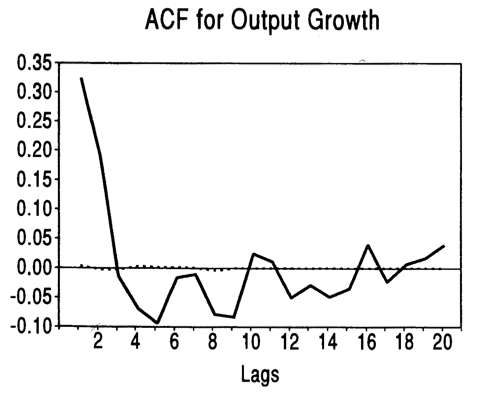
\includegraphics[width=\linewidth]{figures/Bse_ACF.png}
            \caption{Baseline Model}
        \end{figure}

        \column{0.33\textwidth}
        \begin{figure}
            \centering
            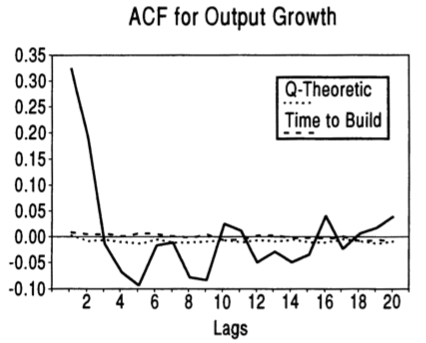
\includegraphics[width=\linewidth]{figures/K_ACF.png}
            \caption{Capital Adjustment Cost}
        \end{figure}

        \column{0.33\textwidth}
        \begin{figure}
            \centering
            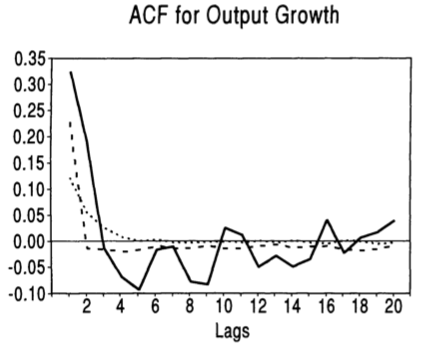
\includegraphics[width=\linewidth]{figures/L_ACF.png}
            \caption{Labor Adjustment Cost}
        \end{figure}
    \end{columns}

    \begin{itemize}
        \item Baseline \& Capital: ACF are close to zero $\Rightarrow$ No serial
              autocorrelation
        \item Labor: Positive autocorrelation at lag 1, and modest negative autocorrelation
              at higher-order lags
    \end{itemize}

\end{frame}

\begin{frame}{Spectrum for Output Growth}
    \begin{columns}[T,onlytextwidth]
        \column{0.33\textwidth}
        \begin{figure}
            \centering
            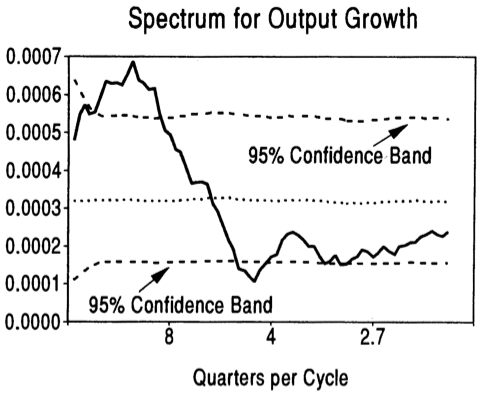
\includegraphics[width=\linewidth]{figures/Base_spect.png}
            \caption{Baseline Model}
        \end{figure}

        \column{0.33\textwidth}
        \begin{figure}
            \centering
            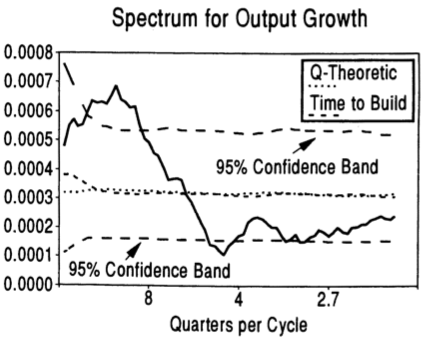
\includegraphics[width=\linewidth]{figures/K_spect.png}
            \caption{Capital Adjustment Cost}
        \end{figure}

        \column{0.33\textwidth}
        \begin{figure}
            \centering
            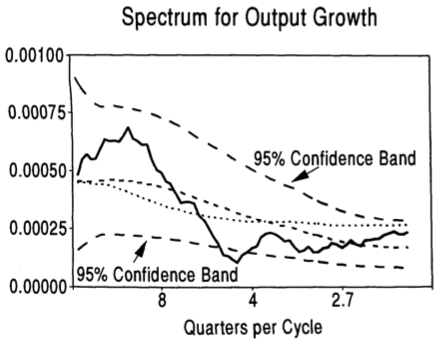
\includegraphics[width=\linewidth]{figures/L_spect.png}
            \caption{Labor Adjustment Cost}
        \end{figure}
    \end{columns}

    \begin{itemize}
        \item Baseline \& Capital: Spectrum is quite flat $\Rightarrow$ No Business-cycle
              periodicity in output growth
        \item Labor: Modest business-cycle periodicity
    \end{itemize}

\end{frame}

\begin{frame}{Permanent Impulse Response Function}
    \begin{columns}[T,onlytextwidth]
        \column{0.33\textwidth}
        \begin{figure}
            \centering
            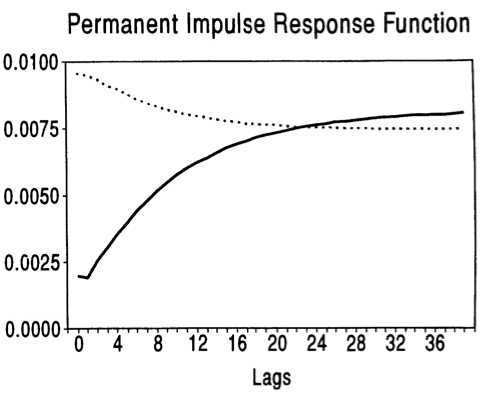
\includegraphics[width=\linewidth]{figures/Base_per_IRF.png}
            \centering\caption{Baseline Model}
        \end{figure}

        \column{0.33\textwidth}
        \begin{figure}
            \centering
            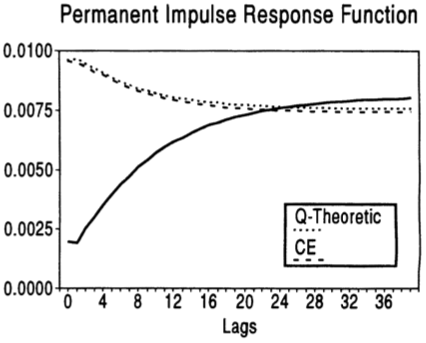
\includegraphics[width=\linewidth]{figures/K_per_IRF.png}
            \centering\caption{Capital Adjustment Cost}
        \end{figure}

        \column{0.33\textwidth}
        \begin{figure}
            \centering
            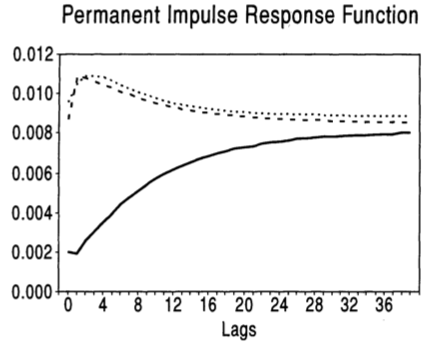
\includegraphics[width=\linewidth]{figures/L_per_IRF.png}
            \centering\caption{Labor Adjustment Cost}
        \end{figure}
    \end{columns}

    \begin{itemize}
        \item Baseline \& Capital: Some success in matching the permanent IRF (at
              higher-order lags)
        \item Labor: Hump-shared response of output to technology shocks
    \end{itemize}

\end{frame}

\begin{frame}{Transitory Impulse Response Function}
    \begin{columns}[T,onlytextwidth]
        \column{0.33\textwidth}
        \begin{figure}
            \centering
            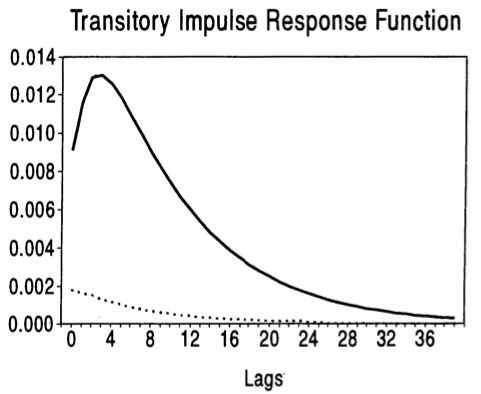
\includegraphics[width=\linewidth]{figures/Base_trans_IRF.png}
            \caption{Baseline Model}
        \end{figure}

        \column{0.33\textwidth}
        \begin{figure}
            \centering
            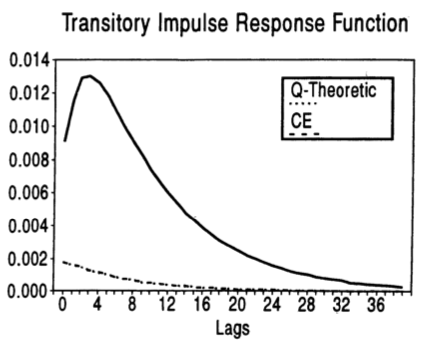
\includegraphics[width=\linewidth]{figures/K_trans_IRF.png}
            \caption{Capital Adjustment Cost}
        \end{figure}

        \column{0.33\textwidth}
        \begin{figure}
            \centering
            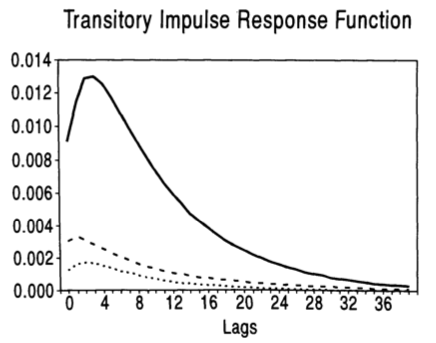
\includegraphics[width=\linewidth]{figures/L_trans_IRF.png}
            \caption{Labor Adjustment Cost}
        \end{figure}
    \end{columns}

    \begin{itemize}
        \item Baseline \& Capital: Wrong qualitative and quantitative response to transitory
              shocks
        \item Labor: Right qualitative response to transitory shocks (small hump), but too
              small in magnitude
    \end{itemize}

\end{frame}

\section{Contribution}

\begin{frame}{Contribution}
    \begin{itemize}
        \item Baseline model and gestation lags and capital adjustment costs model have weak
              internal propagation mechanisms and do not generate dynamics via their internal
              structure
        \item Models that rely on lags or costs of adjusting labor input are partially
              successful:
              \begin{itemize}
                  \item Right pattern of autocorrelation in output growth
                  \item Small hump in transitory IRF
              \end{itemize}
    \end{itemize}

\end{frame}

\begin{frame}{Impulse and Propagation}
    In baseline model, the permanent component of output can be written as
    $$
        y_{\mathrm{P}}(t)=\underbrace{\left[\frac{\varepsilon_{\mathrm{a}}(t)}{1-L}\right]}_{\textit{shock dynamics}}\underbrace{\left[(1.04)\left(\frac{1-0.87 L}{1-0.94 L}\right)\right]}_{\textit{propagation effect}}
    $$

    The transitory component of output can be written as $$
        y_{\mathrm{T}}(t)=\underbrace{\left[\frac{\varepsilon_{\mathrm{g}}(t)}{1-0.96
                    L}\right]}_{\textit{shock dynamics}}\underbrace{(0.16)}_{\textit{propagation
            effect}} $$ $\Rightarrow$ Little contribution from propagation mechanisms

\end{frame}

\begin{frame}{Propagation Mechanism}
    \begin{figure}
        \centering
        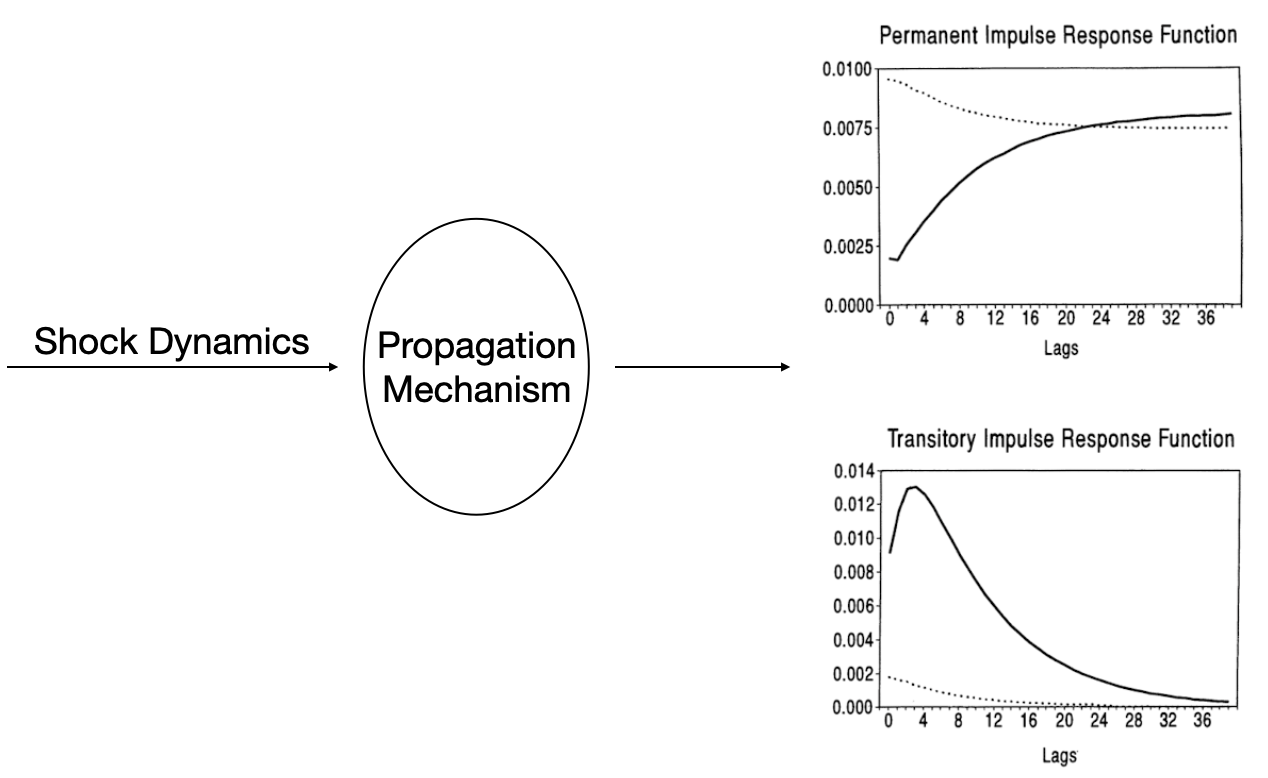
\includegraphics[width=0.8\linewidth]{figures/propagation0.png}
        \caption{Propagation Mechanism}
    \end{figure}

    $\Rightarrow$ Propagation mechanisms in the models do not generate the right kind of output dynamics
\end{frame}

\begin{frame}{Par parentheses}
    In the course example \#3, we have
    \begin{quote}
        RBC model with full depreciation and labor wedge, where $z_t$ follows random walk with drift and $n_t$ follows an AR(1) process.
    \end{quote}
    $\Longrightarrow$ The stochastic components share the same property with those in this paper \cite{cogley_nason_1995}.\\
    $\Longrightarrow$ The model result is also balanced growth, which implies stationarity of $\Delta y_t$ and $n_t$.
    \includegraphics*[width=0.5\textwidth]{figures/example3.png}
\end{frame}

\begin{frame}[allowframebreaks]{References}

    \bibliography{main.bib}
    \bibliographystyle{apalike}

\end{frame}

\end{document}